% Options for packages loaded elsewhere
\PassOptionsToPackage{unicode}{hyperref}
\PassOptionsToPackage{hyphens}{url}
%
\documentclass[
]{article}
\usepackage{amsmath,amssymb}
\usepackage{lmodern}
\usepackage{ifxetex,ifluatex}
\ifnum 0\ifxetex 1\fi\ifluatex 1\fi=0 % if pdftex
  \usepackage[T1]{fontenc}
  \usepackage[utf8]{inputenc}
  \usepackage{textcomp} % provide euro and other symbols
\else % if luatex or xetex
  \usepackage{unicode-math}
  \defaultfontfeatures{Scale=MatchLowercase}
  \defaultfontfeatures[\rmfamily]{Ligatures=TeX,Scale=1}
\fi
% Use upquote if available, for straight quotes in verbatim environments
\IfFileExists{upquote.sty}{\usepackage{upquote}}{}
\IfFileExists{microtype.sty}{% use microtype if available
  \usepackage[]{microtype}
  \UseMicrotypeSet[protrusion]{basicmath} % disable protrusion for tt fonts
}{}
\makeatletter
\@ifundefined{KOMAClassName}{% if non-KOMA class
  \IfFileExists{parskip.sty}{%
    \usepackage{parskip}
  }{% else
    \setlength{\parindent}{0pt}
    \setlength{\parskip}{6pt plus 2pt minus 1pt}}
}{% if KOMA class
  \KOMAoptions{parskip=half}}
\makeatother
\usepackage{xcolor}
\IfFileExists{xurl.sty}{\usepackage{xurl}}{} % add URL line breaks if available
\IfFileExists{bookmark.sty}{\usepackage{bookmark}}{\usepackage{hyperref}}
\hypersetup{
  pdftitle={Serial reversal learning in nectar-feeding bats},
  hidelinks,
  pdfcreator={LaTeX via pandoc}}
\urlstyle{same} % disable monospaced font for URLs
\usepackage[margin=1in]{geometry}
\usepackage{longtable,booktabs,array}
\usepackage{calc} % for calculating minipage widths
% Correct order of tables after \paragraph or \subparagraph
\usepackage{etoolbox}
\makeatletter
\patchcmd\longtable{\par}{\if@noskipsec\mbox{}\fi\par}{}{}
\makeatother
% Allow footnotes in longtable head/foot
\IfFileExists{footnotehyper.sty}{\usepackage{footnotehyper}}{\usepackage{footnote}}
\makesavenoteenv{longtable}
\usepackage{graphicx}
\makeatletter
\def\maxwidth{\ifdim\Gin@nat@width>\linewidth\linewidth\else\Gin@nat@width\fi}
\def\maxheight{\ifdim\Gin@nat@height>\textheight\textheight\else\Gin@nat@height\fi}
\makeatother
% Scale images if necessary, so that they will not overflow the page
% margins by default, and it is still possible to overwrite the defaults
% using explicit options in \includegraphics[width, height, ...]{}
\setkeys{Gin}{width=\maxwidth,height=\maxheight,keepaspectratio}
% Set default figure placement to htbp
\makeatletter
\def\fps@figure{htbp}
\makeatother
\setlength{\emergencystretch}{3em} % prevent overfull lines
\providecommand{\tightlist}{%
  \setlength{\itemsep}{0pt}\setlength{\parskip}{0pt}}
\setcounter{secnumdepth}{-\maxdimen} % remove section numbering
\usepackage{lineno}
\linenumbers
\usepackage{float} \floatplacement{figure}{H}
\newcommand{\beginsupplement}{\setcounter{table}{0}  \renewcommand{\thetable}{S\arabic{table}} \setcounter{figure}{0} \renewcommand{\thefigure}{S\arabic{figure}}}
\usepackage{multirow}
\usepackage{multicol}
\usepackage{colortbl}
\usepackage{hhline}
\usepackage{longtable}
\usepackage{array}
\usepackage{hyperref}
\ifluatex
  \usepackage{selnolig}  % disable illegal ligatures
\fi
\newlength{\cslhangindent}
\setlength{\cslhangindent}{1.5em}
\newlength{\csllabelwidth}
\setlength{\csllabelwidth}{3em}
\newenvironment{CSLReferences}[2] % #1 hanging-ident, #2 entry spacing
 {% don't indent paragraphs
  \setlength{\parindent}{0pt}
  % turn on hanging indent if param 1 is 1
  \ifodd #1 \everypar{\setlength{\hangindent}{\cslhangindent}}\ignorespaces\fi
  % set entry spacing
  \ifnum #2 > 0
  \setlength{\parskip}{#2\baselineskip}
  \fi
 }%
 {}
\usepackage{calc}
\newcommand{\CSLBlock}[1]{#1\hfill\break}
\newcommand{\CSLLeftMargin}[1]{\parbox[t]{\csllabelwidth}{#1}}
\newcommand{\CSLRightInline}[1]{\parbox[t]{\linewidth - \csllabelwidth}{#1}\break}
\newcommand{\CSLIndent}[1]{\hspace{\cslhangindent}#1}

\title{Serial reversal learning in nectar-feeding bats}
\author{}
\date{\vspace{-2.5em}}

\begin{document}
\maketitle

\begin{center}\rule{0.5\linewidth}{0.5pt}\end{center}

\begin{center}\rule{0.5\linewidth}{0.5pt}\end{center}

Shambhavi Chidambaram\textsuperscript{1,2}, Sabine Wintergerst\textsuperscript{3}, Alex Kacelnik\textsuperscript{4}, York Winter\textsuperscript{1,2}, Vladislav Nachev\textsuperscript{1\textbf{*}}

\textsuperscript{1} Institute of Biology, Humboldt University, Berlin, Germany

\textsuperscript{2} Berlin School of Mind and Brain, Humboldt University, Berlin, Germany

\textsuperscript{3} Fairchild Tropical Botanic Garden, 10901 Old Cutler Rd, Miami, FL 33156

\textsuperscript{4} Department of Zoology, University of Oxford

\textsuperscript{\textbf{*}}\textbf{For correspondence:} york.winter@charite.de

\textbf{Present Address:} Institute of Biology, Humboldt University, Philippstr. 13, 10099 Berlin, Germany

\hypertarget{abstract}{%
\section{Abstract}\label{abstract}}

The tropical bat species \emph{Glossophaga commissarisi} mainly feeds on nectar from flowers. Flowering plants stay fixed in one place, but the amount of nectar flowers contain varies as the flowers get emptied, replenish their nectar, or wither and die. Nectar-feeding bats must be capable of perceiving and responding flexibly to these changes in their environment. We aimed to demonstrate this through a spatial serial reversal learning task with wild \emph{G. commissarisi} individuals. The bats were given two options in two places that did not change, one providing a reward, the other providing no reward. Once the bats had experienced the rewading properties of these options for some time, the properties reversed, and this reversal occurred repeatedly. We found that as bats experience serial reversals they show a more rapid switch to the rewarding option after a reversal, and an overall increase in the number of choices for the rewarding option. This overall increase was smaller with each successive reversal, indicating that the preference for the rewarding option was so high it could not increase much further: a ceiling effect. In the trade-off between exploiting options known to be rewarding and exploring new options, the bats' behaviour approached a `best of both worlds' strategy. The bats showed near-exclusive preference for the rewarding option, which they changed rapidly following a reversal. This is strong evidence of `learning to learn,' or learning the rule of the reversals. Additional analyses showed that the highest number of choices for the rewarding option was made every night before the bats had experienced any reversals at all. Rule-learning could only happen after reversals had occurred; before that the bats strongly preferred to visit and exploit the only option known to be rewarding, rather than explore any other option.

\hypertarget{introduction}{%
\section{Introduction}\label{introduction}}

\begin{quote}
`Take some more tea,' the March Hare said to Alice, very earnestly.
\end{quote}

\begin{quote}
`I've had nothing yet,' Alice replied in an offended tone, `so I can't take more.'
\end{quote}

\begin{quote}
`You mean you can't take LESS,' said the Hatter: `it's very easy to take MORE than nothing.'
\end{quote}

\begin{quote}
\hfill *\textbf{Alice\('\)s Adventures in Wonderland}*\textbf{, Lewis Carroll}
\end{quote}

Nectar-feeding bats face the challenge of exploiting a resource that varies in temporal and spatial availability. Flower nectar levels vary within any given night, as well from night to night; flowering plants often bloom seasonally and flowers themselves wither and die every day or every few days. Bats need to detect the changing reward contingencies in their environment and adjust their behaviour accordingly. This ability of animals to recognize and respond to changes is crucial to survival, and includes cognitive or behavioural flexibility (Tello-Ramos et al. 2019). It can be seen in a range of behaviours in many different species: locating food in ants (Czaczkes and Heinze 2015); spatial navigation in male guppies (Lucon-Xiccato and Bisazza 2017) and parental care in poison frogs (Ringler et al. 2015). One experimental protocol that has been widely used to demonstrate cognitive/behavioural flexibility is reversal learning, a task that could be a simple experimental analogue to some of the kinds of decision-making bats do in their natural environment.

Reversal learning is essentially a type of discrimination learning, which is when animals must learn a specific response to each of multiple stimuli. In a reversal learning experiment an animal is first faced with a simultaneous choice between two stimuli. Responding to one stimulus but not the other results in a reward for the animal. After a certain number of trials has occurred and the animal has learned to perform the response that leads to a reward, the reward contingencies of the two stimuli are reversed. In a serial reversal learning procedure the reward contingencies reverse repeatedly. An animal that responds to the rewarding stimulus more frequently than to the non-rewarded stimulus receives food more often, and can be said to perform `better' on the task; a choice to the non-rewarded stimulus is, in the context of the task, an `error.'

The serial reversal learning protocol can be adapted to the behaviour and sensory physiology of many different species, thus allowing comparative research. It has been done using visual stimuli in bumblebees (Strang and Sherry 2014) and guppies (Boussard et al. 2020); visual and spatial stimuli in both corvids (Bond, Kamil, and Balda 2007) and cowbirds (Lois-Milevicich et al. 2021); spatial stimuli in rats (Boulougouris, Dalley, and Robbins 2007), great tits (Hermer et al. 2018a) and gray squirrels (Chow et al. 2015); and olfactory stimuli in rats (Kinoshita et al. 2008). Reversal learning, specifically serial reversal, has been used as an explicit comparative measure of animal `intelligence' (Bitterman 1964): animals considered then to be `higher,' like pigeons, rats and monkeys showed a progressive improvement on the task while species considered to be `lower,' like turtles and fish, did not. Though the idea of such a hierarchy is outdated, comparative research using reversal learning can reveal important differences in behaviour and learning that have evolved under the selection pressures faced by different species.

Improvement in the reversal learning task is clearly demonstrable, and is therefore a meaningful criterion when comparing the performance of different animals. First-order learning happens when an animal perceives a stimulus and learns which behavioural response leads to a reward - the stimulus-reward association - and changes its behaviour according to the strength of this reinforcement. Higher-order or second-order learning is the learning of rules or strategies. This is the ability to more efficiently choose the best response in any given situation, from among many different learned behavioural responses. In serial reversal learning the same stimuli are successively paired with a reward and then not paired with a reward. Under such conditions animals must learn the second-order rule to quickly abandon a suddenly unsuccessful response when it previously resulted in reward. A rule that can maximize reward in a deterministic, fixed ratio reversal learning is `win-stay; lose-shift' (WSLS): repeat the behaviour which produces a reward until it stops being rewarding, and then immediately change the behaviour. Such a rule means in practice that the animal makes exactly one `error' per reversal. After learning the task, the perfectly optimal animal will first exclusively respond to the stimulus that is paired with reward. At the first choice of this stimulus that does not result in reward (the error), the animal will change its preference and exclusively respond to the other stimulus which is now paired with a reward.

Animals are rarely, if ever, so optimal in real life. Large and deterministic changes are uncommon in nature and more gradual shifts in behaviour maybe better suited to natural environmental changes. Errors in a task like fixed-ratio reversal learning are common, and can occur in different ways. An animal can make anticipatory errors: changing their behaviour and choosing the other cue before a reversal has occurred; or they can perseverate: continuing to choose a non-rewarding cue after the reversal has occurred. Progressive `improvement' in this task, where an animal makes fewer and fewer errors per reversal is indication that the animal is learning the rule of reversal, or `learning to learn' (Shettleworth 2010).

Primates show a very interesting difference in between first- and second-order learning. In one study, thirteen different species of primates were compared on a visual reversal learning task (Rumbaugh, Savage-Rumbaugh, and Washburn 1996), where they were trained to discriminate a pair of stimuli up to either a 67\% or 84\% level of correct choices for the rewarded option. At these two different levels of training they were then given a single reversal of reward contingencies. If the primates' behaviour was driven mainly by first-order learning, they should switch to the newly-rewarding stimulus more quickly when their training had not yet reached a high level of performance, i.e., 67\%. The opposite would be true if second-order learning or rule-learning was occurring: knowing the reversal rule, the primates would more quickly adapt to the reversed option when they had reached a high level of performance in their training, i.e., 84\%. The results showed that Prosimian species tended to perform better when trained to 67\% and apes when trained to 84\% level of correct choices before the reversal.

Progressive improvement on the serial reversal task as more reversals are experienced, which is evidence of rule-learning, has been shown in many different species: bumblebees (Strang and Sherry 2014); great tits from different environments (Hermer et al. 2018a); three different species of corvids (Bond, Kamil, and Balda 2007); rats (Castañé, Theobald, and Robbins 2010); and marmosets (Clarke, Robbins, and Roberts 2008). A decrease in the number of errors to reach a criterion (a pre-decided number of correct choices) with multiple reversals is seen in mice (Caglayan, Stumpenhorst, and Winter 2021), even when each reversal is done with a different pair of stimuli, indicating the formation of a learning set.

What performance on the serial reversal task says about the deeper cognitive mechanisms at work, and whether the task is a measure of cognitive or behavioural flexibility, are not completely settled questions. Cognitive flexibility cannot be directly observed; it is inferred to have occurred through changes in behaviour, or behavioural flexibility (Tait et al. 2018). However, behavioural flexibility does not necessarily indicate cognitive flexibility (Dhawan, Tait, and Brown 2019). The term `behavioural flexibility' itself has been used widely but inconsistently, applied to many traits that have different underlying neural mechanisms or do not co-vary (Audet and Lefebvre 2017). Behavioural flexibility in animals has evolved in response to selection pressures from different foraging environments: the flexibility required to deal with seasonal changes in fruit availability is not the same kind of flexibility required to deal with capturing a prey animal intent on escaping.

There is a sense in which the foraging ecology of some nectar-feeding animals is a natural analogue to the serial reversal learning task. The Neotropical bat species \emph{Glossophaga commissarisi} relies primarily on flower nectar for energy. These bats have remarkably high metabolic rates for their body mass (Voigt and Winter 1999; Voigt, Kelm, and Visser 2006), due to the energetic demands of hovering flight (Y. Winter and Helversen 1998; Helversen and Reyer 1984). Many plants visited by bats put out only a few flowers every night, but their flowering seasons that can last for several months. Bat-pollinated flowers can secrete up to 1-2 mL of nectar a night (Helversen 1993) but as only small droplets are available each time they are visited (Voigt, Kelm, and Visser 2006), the bats make several hundred flower visits per night. Indeed, a certain time after a flower is emptied the nectar-levels are replenished, so bats can visit the same flower multiple times. The bats relocate the flowering plant primarily through their excellent spatial memory (York Winter and Stich 2005), and use local echo-acoustic cues to find the individual flowers (Tölch et al. 2008). The longer the bat waits, the more the flower refills but the higher the likelihood that a competitor could find and exploit the flower first. To make repeated, profitable visits to a flower, a bat must remember both the location of the flower and estimate the flower's expected reward value. The serial reversal learning task requires an animal to respond to a change in the profitability of available options, and remember all potentially rewarding options. Though this is a simplified situation with no inter-individual competition and where the `flowers' do not get progressively depleted, the behavioural flexibility required by the experimental protocol is the kind of flexibility required in the natural foraging circumstances of a nectar-feeding bat.

We carried out a serial reversal learning task with wild \emph{G. commissarisi} individuals. The bats were given two potentially rewarding options to choose between. At the start of the night, only one of the options was rewarding, the `S+' option and the other was not rewarding, the `S-' option. After a certain number of visits had been made by the bats, the reward contingencies reversed without any signal or cue to the bats: the previously rewarding option was now unrewarding and the previously unrewarding option was rewarding, and this reversal happened five times in a night.

Our aims with this experiment were as follows. Firstly, we wanted to test whether the bats would alter their preference between the two reward sources accordingly to their transient rewarding properties. We believed this to be extremely likely as the behavioural requirements of the task reproduce aspects of the animals' foraging ecology. Flowers that have remained undetected and are full of nectar will also require multiple visits for depletion. Secondly, if the bats demonstrated flexibility through an ability to respond to the reversals, we wanted to explore how this was reflected in their decision-making. What would be the relative number of visits made to the rewarding and the non-rewarding options, and how swiftly would allocation change after a reversal? Thirdly, we wanted to see if the bats were capable of second-order learning, or `learning to learn.' Could the bats learn the rule behind the change in their environment and converge to the maximal payoff of one error per reversal achievable through WSLS?

After the analyses described above were done and the data and results examined, we performed further analyses to explore the conclusions of our confirmatory analyses. The difference between these results must be clearly noted. Firstly, we reasoned that there is a difference between the first visits of a night, before any experience of a change in contingencies, and all the subsequent visits after at least one reversal had occurred. We statistically tested for this difference in the bats' choice behaviour. Secondly, we examined the effect of the asymptotic level of performance (the highest stable proportion of visits to the rewarding option) on the performance immediately after a reversal.

\hypertarget{methods}{%
\section{Methods}\label{methods}}

\hypertarget{study-site-and-subjects}{%
\subsection{Study site and subjects}\label{study-site-and-subjects}}

The experiment took place from the 28th of June to the 25th of July, 2017, at La Selva Biological Field Station, Province Heredia, Costa Rica. Bats of the species \emph{Glossophaga commissarisi} were captured from the wild and retained in a flight cage through the experiment. The bats were attracted to a particular location in the forest using sugar-water (see \textbf{Reward} below) as bait and then caught in mist-nets. The bats were sexed on capture and housed in two outdoor, meshed flight-cages (4 x 6 m) under ambient light conditions. All individuals were weighed and marked with radio frequency identification (RFID) tags placed as collars around their necks.

16 bats participated in the main experiment. At the end of the experiment, the RFID collars were removed and the bats were released back into the wild . All the data collection was completely automatized. Two of the bats did not drink a sufficient amount of sugar-water to meet minimum energy requirements and were released before the end of the experiment and not replaced. The data from these two individuals were not analyzed. Thus, 14 bats (seven males and seven females) completed the experiment.

Animal experimental procedures were reviewed and permission was granted by Sistema Nacional de Areas de Conservación (SINAC) at the Ministerio de Ambiente y Energía (MINAE), Costa Rica.

\hypertarget{experimental-setup}{%
\subsection{Experimental Setup}\label{experimental-setup}}

\hypertarget{reward}{%
\subsubsection{Reward}\label{reward}}

The reward received by the bats during the experiment was also their main source of food. The reward was a 17\% by weight solution of sugar dissolved in water, hereafter referred to as `nectar.' The sugar consisted of a 1:1:1 mass-mixture of sucrose, fructose and glucose. The nectar was thus similar in composition and concentration to the nectar produced by wild chiropterophilous plants (Baker, Baker, and Hodges 1998).

\hypertarget{flower-and-pump-setup}{%
\subsubsection{Flower and pump setup}\label{flower-and-pump-setup}}

Each flight cage had a square plastic frame in the center (2x2x1.5m). Eight reward-dispensing devices - hereafter referred to as `flowers' - were fixed in a radial pattern on this frame, two on each side of the square (see Figure \ref{fig:Pump-pictures}) with a distance of 40 cm between adjacent flowers. At this distance bats can easily discriminate neighbouring flowers (Thiele and Winter 2005). Each flower had the following parts: an RFID reader mounted on a plastic cylinder around the head of the flower; an infra-red light-barrier beam; an electronic pinch valve through which a silicon tube was placed and fixed to the head of the flower.

A stepper-motor pump was placed in the center of the plastic frame in each cage. The pumps contained a 25 mL Hamilton glass syringe (Sigma Aldrich). The step volume of the two pumps differed slightly: the pump in Cage 1 delivered 2.11 \(\mu\)L per step of the stepper-motor, and the pump in Cage 2, 3.33 \(\mu\)L per step. The glass syringe was connected to the tubing system of the flowers through five pinch valves. The pinch valves controlled the flow of liquid from the pump to the system and from a reservoir of liquid to the pump. The reservoir (500 mL thread bottle, Roth, Germany) was filled with fresh nectar everyday and connected to the syringe through the valves.

When a tagged bat approached a flower, the individual RFID number was read by the reader. If the bat then poked its nose into the flower and broke the light barrier, it triggered the release of a reward. The pinch valve opened and the pump moved the correct number of pre-programmed steps to dispense nectar to the head of the flower. The bat could easily hover in front of the flower and lick up the nectar. Only when both events occurred, i.e., the RFID reader identified a bat and the light-barrier was broken, would a reward be triggered. The flowers and the pump were connected to a laptop computer with Windows operating system, which ran the experimental programs and the program used to clean and fill the systems: PhenoSoft Control (PhenoSys GmbH, Berlin, Germany). The raw data were recorded as comma-separated value (CSV) files.



\begin{figure}[H]

{\centering 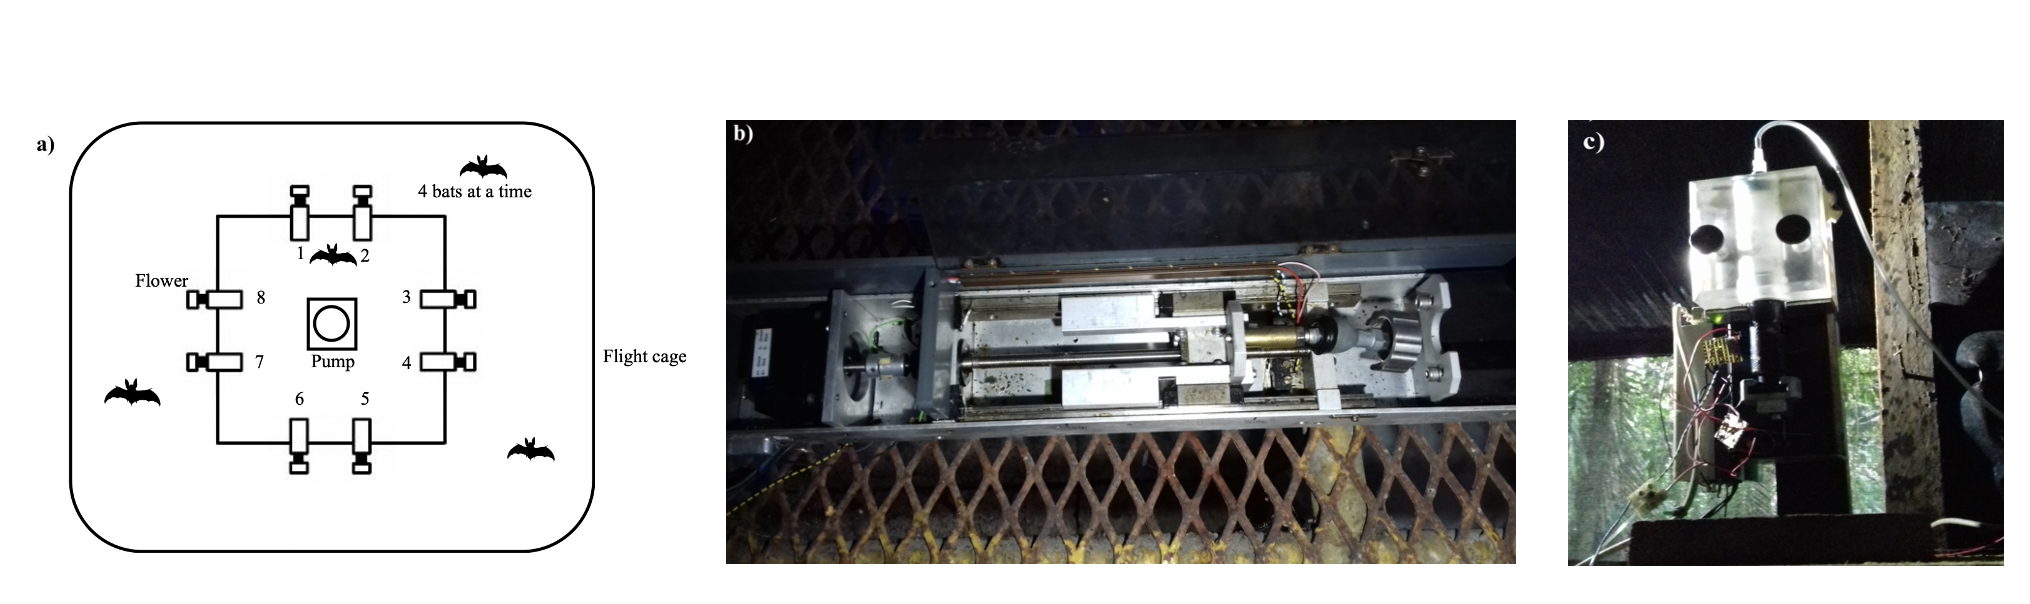
\includegraphics[width=28.19in]{images/allthree} 

}

\caption{a) Schematic of the cage and flower set-up b) Pump in cage 1 c) Pump in cage 2}\label{fig:Pump-pictures}
\end{figure}

\hypertarget{experimental-procedure}{%
\subsection{Experimental procedure}\label{experimental-procedure}}

Every day at around 1000 h the old nectar was emptied from the system. The system was rinsed and filled with plain water until 1500 h, when it was filled again with fresh nectar. Twice a week the system was filled with 70\% ethanol for an hour to prevent microbial growth, then repeatedly rinsed with water.

Four bats of the same sex were placed in a flight-cage in a group. There were four such groups in total, and data were collected simultaneously from two groups, one in each flight-cage. Each bat was uniquely assigned two adjacent flowers on the same side of the square frame, out of the array of eight. These flowers were programmed to reward to only one of the four bats in the cage. After the system was filled with fresh nectar at approximately 1700 h, the program was left running for data-collection till the next morning. Thus, the bats could begin visiting the flowers to collect a reward whenever they chose, which was at nightfall at approximately 1800 h every night.

During the course of the night, when the syringe of the pump had been emptied, the pump re-filled automatically. This event happened only once every night. On the main experimental days this process took 4.49 minutes (SD = ±0.18) for the horizontal pump, and 2.42 minutes (SD = ±0.04) for the vertical pump.

About 1 \% (SD = ±0.74) of all visits made by the bats over all three experimental nights were wrongly unrewarded: the bats did not receive a reward during these visits even when they were made to a flower assigned to them that was rewarding at the time. This happened either during the pump refill times or when the pump was moving to reward a visit made by another bat that happened almost at the same time, and did not count towards the total of 50 visits in a block.

Every night the bats were also given ad-libitum access to supplemental food: 3.5g of hummingbird food (NektarPlus, Nekton) and 3.5g of milk powder (Nido 1+, Nestle) in 10 mL of water. They were also given a small bowl of locally-sourced bee pollen.

\hypertarget{experimental-design}{%
\subsection{Experimental design}\label{experimental-design}}

The experiment proceeded through the following stages.

\hypertarget{training}{%
\subsubsection{Training}\label{training}}

On the night the naive bats were captured and placed into the flight cages they could receive a reward from any of the flowers whenever they visited them throughout the night. To enable the bats to find the flowers a small cotton pad was placed on the flowers, soaked in di-methyl di-sulphide. This is a chemical attractant produced by many bat-pollinated flowers (Helversen, Winkler, and Bestmann 2000). A small drop of honey was applied to the inside of the flowers to encourage the bats to place their heads inside, break the light-barrier and trigger a nectar reward. By the end of the night all the bats had found the flowers and learned to trigger rewards.

After the bats had learned to trigger rewards, the next stage of training involved assigning the bats uniquely to two out of the eight flowers in the array. For an individual animal only the two flowers assigned to it would be rewarding from this stage of training until the end of the experiment. This stage was similar to the previous one, except the bats could only trigger a reward at their assigned flowers, and the chemical attractant and honey were not used.

To ensure that the bats were familiar with both flowers assigned to them they went through one final stage of training: forced alternation after each reward between the two assigned flowers all night long.

\hypertarget{serial-reversal-learning-task}{%
\subsubsection{Serial Reversal Learning Task}\label{serial-reversal-learning-task}}

In the serial reversal learning task the bats had continuous access to two flowers, one that gave a 40 \(\mu\)L nectar reward and one that was empty. The location of the rewarding flower was not cued, but through the Alternation phase of training each bat knew the locations of both flowers that were potentially rewarding to it. After a bat had made 50 visits in total to the two flowers (regardless of relative allocation) a reversal occurred: the previously rewarding flower became the non-rewarding flower and \emph{vice versa}. Importantly, only visits to the two flowers assigned to a bat counted towards the visit tally, not visits to any of the other flowers in the flight cage which were always unrewarding to that particular bat. Each batch of 50 visits to the assigned two flowers, either at the start of each night or between reversals, was termed a `reversal block.' There were six blocks and five reversals per night, unless the bat ceased visiting earlier. This was repeated for three consecutive nights. The same flower started the sequence every night. Consequently the last flower to be rewarding one night was non-rewarding at the start of the next.

\hypertarget{data-analysis}{%
\subsection{Data analysis}\label{data-analysis}}

All the models were fitted in a Bayesian framework using Hamiltonian Monte Carlo in the R package \texttt{brms} (Bürkner 2017), which is a front-end for \texttt{rstan} (Stan Development Team, 2020). Model comparison was done using leave-one-out cross-validation, implemented in \texttt{brms} using the package \texttt{loo} (Vehtari, Gelman, and Gabry 2017).

Except when stated otherwise, all the visits made by the bats to their two assigned flowers - up to 300 -- during a night were included in the analyses (some of the bats did not complete all 300 visits on every night). The bats made some visits and approaches to the flowers that were not assigned to them but they were the minority, and not considered for the analysis (see \textbf{Supplementary Information} for details). At the end of each of the first five blocks a reversal occurred and the end of the last block was the end of data-collection for the night. Each block was further divided into five bins of ten visits, in order to examine the bats' behaviour within each block. Generalized linear mixed-models were used for the analyses (see \textbf{Supplementary Information} for details of the model fitting). We report here the mean as a measure of central tendency and the 89\% quantile-based credible intervals for the parameters. (89\% boundaries are the default for reporting credible intervals and are no more arbitrary than the convention of using 89\% boundaries - (McElreath 2020))

We investigated the effect of experimental night and reversal block on the number of perseverative visits, i.e., visits to the previously-rewarding option just after the occurrence of a reversal; and the effect of experimental night, block and bin on the proportion of visits to the rewarding flower. The proportion of visits to the rewarding flower was calculated as the number of visits to the S+ divided by total number of visits to both the S+ and S-, and we denote this as the preference index or I\textsubscript{pref}:

\[\mathrm{I_{pref}} = \displaystyle \frac{\rm Number \;of\; visits\; to\; the\; S+}{\rm (Number \;of\; visits\; to\; the\; S+) + (\rm Number \;of\; visits\; to\; the\; S-)}\]

After examining the these results, we conducted further post-hoc exploratory analyses. Firstly, we investigated the effect of night, block, bin, and the first night and first block of the night as separate predictor variables for I\textsubscript{pref}: on the first night the animals had had no prior experience of any reversals, and during the first block of every night they had not experienced any reversals on that night. Secondly, we compared the I\textsubscript{pref} in the three bins just before a reversal (the asymptote) and the number of visits just after a reversal as we thought this might reveal something of the learning mechanisms at work.

All statistical analyses and creation of plots were done in R.

\hypertarget{data-availability}{%
\subsection{Data availability}\label{data-availability}}

All data and analysis code are available online at \ldots..

\hypertarget{results}{%
\section{Results}\label{results}}

\hypertarget{confirmatory-analyses}{%
\subsection{Confirmatory Analyses}\label{confirmatory-analyses}}

\hypertarget{a-bats-made-a-very-high-proportion-of-their-visits-to-the-rewarding-option}{%
\subsubsection{a) Bats made a very high proportion of their visits to the rewarding option}\label{a-bats-made-a-very-high-proportion-of-their-visits-to-the-rewarding-option}}



\begin{figure}[H]

{\centering \includegraphics{srl_complete_210527_files/figure-latex/overall-summary-1} 

}

\caption{Visits to the rewarding option across the three experimental nights. Data are average proportions for bins of ten visits averaged over all individuals. Data are indicated by white points in the first block on the first night before the bats experienced any reversals at all; the bin averages of all the other blocks are indicated by black points. Numbers indicate the bats that participated in a particular reversal block. Shading shows 95\% confidence intervals. Dashed lines show reversals.}\label{fig:overall-summary}
\end{figure}

The allocation of visits between each bat's two flowers is shown in Figure \ref{fig:overall-summary}. Of particular interest is what the bats did in the first bins of each block, and the changes between the first night and the other two nights. At the start of the first night, in the very first bin of ten visits when the bats did not yet have any information about the available options and had never experienced a reversal, the I\textsubscript{pref} averaged across individuals was close to chance: 54.5\% {[}95\% CI 46.1, 62.3{]}. Within the next ten visits, however, I\textsubscript{pref} increased to 92.1\% {[}95\% CI 87.1, 96.4{]} and by the last bin of this first block was 99.3\% {[}95\% CI 97.9, 100{]}. Immediately after the first experience of a reversal, the I\textsubscript{pref} dropped down to 13.6\% {[}95\% CI 8.4, 18.8{]} in the first ten visits, but came back up to 96.4\% {[}95\% CI 92.9, 99.3{]} by the last bin of this block.

This pattern of a decrease in the average proportion of visits to the rewarding option of all the bats immediately following a reversal, and then a rapid increase, was consistently true for all the reversals on the first night. At the very start of the second and third nights, in the first bin of visits before any experience of a reversal on that night, the average I\textsubscript{pref} of all the bats was 69.8\% {[}95\% CI 64.3, 75{]}. However the I\textsubscript{pref} still showed the pattern of a decrease immediately after a reversal and then increase to a high proportion - 94.8\% {[}95\% CI 94.1, 95.5{]}, comparable to the 93\% {[}95\% CI 91.8, 94.2{]} on the first night.

\hypertarget{b-bats-switch-to-the-rewarding-option-faster-as-they-experience-more-reversals}{%
\subsubsection{b) Bats switch to the rewarding option faster as they experience more reversals}\label{b-bats-switch-to-the-rewarding-option-faster-as-they-experience-more-reversals}}

We called the run of consecutive visits to a non-rewarding flower immediately after each reversal (before experiencing any reward in that block) perseverative visits. Errors in the first block were not, by definition, treated as perseverative errors. A generalized linear mixed-model was used to investigate the effect of experimental night and reversal block on the number of perseverative visits. A negative-binomial likelihood function was used for this model. Experimental night, reversal block and their interaction were fixed effects and random slopes and intercepts were used to fit regression lines for each individual animal.

We called the run of consecutive visits to a non-rewarding flower immediately after each reversal (before experiencing any reward in that block) perseverative visits. Both experimental night (1 to 3) and block (1 to 5) had a negative effect on the number of perseverative visits made by the bats. As the bats experienced more reversals on more nights the number of perseverative visits decreased. The effect of the interaction of night and block, however, was positive: perseverative visits decreased less as the bats experienced more experimental nights (Figure \ref{fig:perseverative-visits} and Figure \ref{fig:pers-forest-plot}).



\begin{figure}[H]

{\centering \includegraphics{srl_complete_210527_files/figure-latex/perseverative-visits-1} 

}

\caption{Number of perseverative visits made by the bats after each reversal across all three nights. A perseverative visit was defined as visit to the previously-rewarding option directly after a reversal and before the first visit to the newly-rewarding option. By definition there were no perseverative visits in the first block of a night. The red lines are the perseverative visits made by the individual bats after each reversal of a night; the black lines are the number of perseverative visits averaged over the bats (N = 14). Reversals were between the two flowers assigned to an individual bat}\label{fig:perseverative-visits}
\end{figure}



\begin{figure}[H]

{\centering \includegraphics{srl_complete_210527_files/figure-latex/pers-forest-plot-1} 

}

\caption{Forest plot of the estimates of the effect of night and block on perseverative visits; a negative value indicates a decrease of perseverative visits with successive nights and blocks. Circles represent slope estimates, thick horizontal lines represent 50\% credible intervals, and thin horizontal lines 89\% credible intervals. Numbers are slope estimates and 89\% credible intervals of each effect}\label{fig:pers-forest-plot}
\end{figure}



\begin{figure}[H]

{\centering \includegraphics{srl_complete_210527_files/figure-latex/unnamed-chunk-1-1} 

}

\caption{A comparison of the posterior predictions of the generalized linear mixed-effects model of the perseverative visits (blue line, shading indicates 89\% credible intervals) and the empirical data from the bats (red line)}\label{fig:unnamed-chunk-1}
\end{figure}

\hypertarget{c-after-the-experience-of-reversals-the-bats-make-more-visits-to-the-rewarding-option}{%
\subsubsection{c) After the experience of reversals the bats make more visits to the rewarding option}\label{c-after-the-experience-of-reversals-the-bats-make-more-visits-to-the-rewarding-option}}

The proportion of visits to the rewarding option, the I\textsubscript{pref}, calculated only over the two flowers assigned to each bat, was modeled as an effect of experimental night, block and bin within block. The model was fit using a binomial likelihood function, with experimental night, block, bin and their interactions as fixed effects; random slopes and intercepts were used to fit regression lines for the individuals.

This analysis showed that all three, night, block and bin all had a positive effect on the I\textsubscript{pref}: as the bats experienced more reversals on more nights, and the more visits made since the occurrence of a reversal, the proportion of visits made to the rewarding option increased. Interestingly, the coefficients of the interactions of experimental night and block; block and bin within the block; and experimental night and bin within the block were all negative. In other words, the proportion of visits to the rewarding flower increased, but this increase became smaller as the bats experienced more reversals on more nights. There was a progressively smaller `improvement' in performance, likely through a ceiling effect, given how high the proportion of visits to the rewarding option was (Figure \ref{fig:overall-summary} and Figure \ref{fig:forest-day-block-bin}).



\begin{figure}[H]

{\centering \includegraphics{srl_complete_210527_files/figure-latex/forest-day-block-bin-1} 

}

\caption{Forest plot of the estimates of the effect of night, block and bin on the proportion of visits to the rewarding option; a positive effect indicates the visits to the rewarding option increased with successive nights, blocks and bins (within each block). Circles show slope estimates, thick horizontal lines the 50\% credible intervals and thin horizontal lines the 89\% credible intervals. Numbers are slope estimates with 89\% credible intervals}\label{fig:forest-day-block-bin}
\end{figure}



\begin{figure}[H]

{\centering \includegraphics{srl_complete_210527_files/figure-latex/posterior-day-block-bin-1} 

}

\caption{A comparison of the posterior predictions of the generalized linear mixed-effects model of the visits to the rewarding option and the empirical data from the bats. The red line indicates the average proportion of visits to the rewarding option per bin made by the individual bats, with the red shading indicating 95\% confidence intervals; the blue line indicates the corresponding posterior prediction of the model}\label{fig:posterior-day-block-bin}
\end{figure}

\hypertarget{further-exploratory-analyses}{%
\subsection{Further exploratory analyses}\label{further-exploratory-analyses}}

\hypertarget{a-the-effect-of-the-first-experimental-night-and-the-first-block-of-each-night}{%
\subsubsection{a) The effect of the first experimental night and the first block of each night}\label{a-the-effect-of-the-first-experimental-night-and-the-first-block-of-each-night}}

The first block of an experimental night was qualitatively different from the other blocks, as this was the only part of the night when the bats had not yet experienced a reversal. A similar argument can be made about the first experimental night: on this night the bats experience reversals for the first time. Our confirmatory analyses did not seem to completely capture the effects of experimental night, block and bin. Therefore, we performed an exploratory analysis to specifically explore the effects of the first block and the first night. The GLMM used in this analysis was identical to the that used to investigate the effect of block, bin and night on the I\textsubscript{pref}, except for the addition of experimental night and block as factor variables. The first night and the first block of every night was treated as one level of the factor variables and the other nights and other blocks of each night as the other level.

The main effects of night, block and bin, and their interactions were similar to the previous model (Figure \ref{fig:forest-plot-first-night-first-block}). Additionally, we found that the bats made more visits to the rewarding flower in the first block of every night, before they had experienced any reversal at all: the variable `block type,' (i.e., whether a block was the first reversal block of the night or not), had a positive coefficient. The I\textsubscript{pref} was not any higher on the first night than the other nights, meaning that `night type' did not have an effect. However, the highest I\textsubscript{pref} was in the first block of 50 visits of the first night, before any reversals had ever been experienced even once, compared to any other block on any other night. This was despite the random performance of the very first ten visits (see also Figure \ref{fig:overall-summary}). Thus block type and night type had an interaction effect with a positive coefficient.



\begin{figure}[H]

{\centering \includegraphics{srl_complete_210527_files/figure-latex/forest-plot-first-night-first-block-1} 

}

\caption{Forest plot of the estimates of the effect of night, block, and bin; and the differential effect of the first night and the first block (`night-type' and `block-type') on the proportion of visits to the rewarding option; a positive effect indicates the visits to the rewarding option increased with successive nights, blocks and bins (within each block), or there were more visits to the rewarding option on the `block-type' or `night-type' indicated. The circles represent the slope estimates, the thick horizontal lines represent the 50\% credible intervals and the thin horizontal lines 89\% credible intervals}\label{fig:forest-plot-first-night-first-block}
\end{figure}



\begin{figure}[H]

{\centering \includegraphics{srl_complete_210527_files/figure-latex/posterior-first-block-first-night-1} 

}

\caption{A comparison of the posterior predictions of the exploratory generalized linear mixed-effects model of the visits to the rewarding option and the empirical data from the bats, including the effect of `night-type' and `block-type.' The red line indicates the average proportion of visits to the rewarding option per bin made by the individual bats to show the change, with the red shading indicating 95\% confidence intervals; the blue line indicates the corresponding posterior prediction of the model. Note the differences to Figure \ref{fig:posterior-day-block-bin}: there is a better fit to the data from the first block, especially on Nights 1 and 2 for many of the bats}\label{fig:posterior-first-block-first-night}
\end{figure}

We compared the predictive accuracy of the model that included night type and block type to the model that did not include these, using leave-one-out cross-validation (LOO). The LOO criterion was lower for the former than the latter, indicating better predictive accuracy of the model including night-type and block-type (Table \ref{tab:Model-comparison}). Indeed, its posterior predictions were a better fit for the first block of a night for many of the bats than those of the model that did not include them (Figure \ref{fig:posterior-day-block-bin}).

\providecommand{\docline}[3]{\noalign{\global\setlength{\arrayrulewidth}{#1}}\arrayrulecolor[HTML]{#2}\cline{#3}}

\setlength{\tabcolsep}{2pt}

\renewcommand*{\arraystretch}{1.5}

\begin{longtable}[c]{|p{1.50in}|p{1.50in}|p{1.50in}}

\caption{Comparison of the two models of the proportion of visits to the rewarding option using leave-one-out cross-validation}\label{tab:Model-comparison}\\

\hhline{>{\arrayrulecolor[HTML]{666666}\global\arrayrulewidth=2pt}->{\arrayrulecolor[HTML]{666666}\global\arrayrulewidth=2pt}->{\arrayrulecolor[HTML]{666666}\global\arrayrulewidth=2pt}-}

\multicolumn{1}{!{\color[HTML]{000000}\vrule width 0pt}>{\centering}p{\dimexpr 1.5in+0\tabcolsep+0\arrayrulewidth}}{\fontsize{11}{11}\selectfont{\textcolor[HTML]{000000}{\textbf{Model}}}} & \multicolumn{1}{!{\color[HTML]{000000}\vrule width 0pt}>{\centering}p{\dimexpr 1.5in+0\tabcolsep+0\arrayrulewidth}}{\fontsize{11}{11}\selectfont{\textcolor[HTML]{000000}{\textbf{Difference\ in\ LOO\ estimates}}}} & \multicolumn{1}{!{\color[HTML]{000000}\vrule width 0pt}>{\centering}p{\dimexpr 1.5in+0\tabcolsep+0\arrayrulewidth}!{\color[HTML]{000000}\vrule width 0pt}}{\fontsize{11}{11}\selectfont{\textcolor[HTML]{000000}{\textbf{Standard\ error}}}} \\

\noalign{\global\setlength{\arrayrulewidth}{2pt}}\arrayrulecolor[HTML]{666666}\cline{1-3}

\endfirsthead

\hhline{>{\arrayrulecolor[HTML]{666666}\global\arrayrulewidth=2pt}->{\arrayrulecolor[HTML]{666666}\global\arrayrulewidth=2pt}->{\arrayrulecolor[HTML]{666666}\global\arrayrulewidth=2pt}-}

\multicolumn{1}{!{\color[HTML]{000000}\vrule width 0pt}>{\centering}p{\dimexpr 1.5in+0\tabcolsep+0\arrayrulewidth}}{\fontsize{11}{11}\selectfont{\textcolor[HTML]{000000}{\textbf{Model}}}} & \multicolumn{1}{!{\color[HTML]{000000}\vrule width 0pt}>{\centering}p{\dimexpr 1.5in+0\tabcolsep+0\arrayrulewidth}}{\fontsize{11}{11}\selectfont{\textcolor[HTML]{000000}{\textbf{Difference\ in\ LOO\ estimates}}}} & \multicolumn{1}{!{\color[HTML]{000000}\vrule width 0pt}>{\centering}p{\dimexpr 1.5in+0\tabcolsep+0\arrayrulewidth}!{\color[HTML]{000000}\vrule width 0pt}}{\fontsize{11}{11}\selectfont{\textcolor[HTML]{000000}{\textbf{Standard\ error}}}} \\

\noalign{\global\setlength{\arrayrulewidth}{2pt}}\arrayrulecolor[HTML]{666666}\cline{1-3}\endhead



\multicolumn{1}{!{\color[HTML]{000000}\vrule width 0pt}>{\centering}p{\dimexpr 1.5in+0\tabcolsep+0\arrayrulewidth}}{\fontsize{11}{11}\selectfont{\textcolor[HTML]{000000}{\textbf{Model\ accounting\ for\ the\ first\ night\ and\ first\ block\ separately}}}} & \multicolumn{1}{!{\color[HTML]{000000}\vrule width 0pt}>{\centering}p{\dimexpr 1.5in+0\tabcolsep+0\arrayrulewidth}}{\fontsize{11}{11}\selectfont{\textcolor[HTML]{000000}{0.00}}} & \multicolumn{1}{!{\color[HTML]{000000}\vrule width 0pt}>{\centering}p{\dimexpr 1.5in+0\tabcolsep+0\arrayrulewidth}!{\color[HTML]{000000}\vrule width 0pt}}{\fontsize{11}{11}\selectfont{\textcolor[HTML]{000000}{0.00}}} \\





\multicolumn{1}{!{\color[HTML]{000000}\vrule width 0pt}>{\centering}p{\dimexpr 1.5in+0\tabcolsep+0\arrayrulewidth}}{\fontsize{11}{11}\selectfont{\textcolor[HTML]{000000}{\textbf{Night\ and\ block\ as\ continuous\ only}}}} & \multicolumn{1}{!{\color[HTML]{000000}\vrule width 0pt}>{\centering}p{\dimexpr 1.5in+0\tabcolsep+0\arrayrulewidth}}{\fontsize{11}{11}\selectfont{\textcolor[HTML]{000000}{-108.21}}} & \multicolumn{1}{!{\color[HTML]{000000}\vrule width 0pt}>{\centering}p{\dimexpr 1.5in+0\tabcolsep+0\arrayrulewidth}!{\color[HTML]{000000}\vrule width 0pt}}{\fontsize{11}{11}\selectfont{\textcolor[HTML]{000000}{14.14}}} \\

\noalign{\global\setlength{\arrayrulewidth}{2pt}}\arrayrulecolor[HTML]{666666}\cline{1-3}

\end{longtable}

\hypertarget{b-the-effect-of-asymptotic-performance-on-the-visits-to-the-rewarding-option-just-after-a-reversal}{%
\subsubsection{b) The effect of asymptotic performance on the visits to the rewarding option just after a reversal}\label{b-the-effect-of-asymptotic-performance-on-the-visits-to-the-rewarding-option-just-after-a-reversal}}

We reasoned that a comparison of the bats' behaviour just before and after a reversal might reveal something of the learning mechanisms at work. If a higher I\textsubscript{pref} just before a reversal is predictive of a I\textsubscript{pref} just after, that might potentially indicate that the bats are learning the `rule' behind the reversals and reversing faster. On the other hand, if there is no rule-learning, and the animals' choice is driven by how much reinforcement was received at each option, we would expect the opposite: the I\textsubscript{pref} before the reversal is predictive of a lower I\textsubscript{pref} just after as the reversal from a highly reinforced option is slower. We took the I\textsubscript{pref} averaged over the last three bins of a reversal block for each individual as the `asymptote' of the bats' behaviour. We fit a generalized linear-mixed model with the I\textsubscript{pref} in the first bin just after a reversal as the response variable with the fixed effects asymptote, a continuous variable, and night, a factor variable. Random slopes and intercepts were used to fit regression lines for each individual animal.

Figure \ref{fig:slopes-asymptote-postrev} shows the distribution of the slopes of the regression lines for each bat, with asymptotic I\textsubscript{pref} as the predictor variable and the I\textsubscript{pref} in the bin just after the reversal as the response variable. The more positive this slope, the faster the bats reversed from one option to another.



\begin{figure}[H]

{\centering \includegraphics{srl_complete_210527_files/figure-latex/slopes-asymptote-postrev-1} 

}

\caption{Distribution of the slopes of the regression lines fit for each individual bat for the effect of asymptotic I\textsubscript{pref} on the I\textsubscript{pref} just after the reversal. More positive slopes indicated that a higher preference for the S+ before the reversal was also indicative of a higher preference after the reversal, or a faster reversal. A negative slope indicated the opposite, i.e., a slower reversal. The three experimental nights are indicated by the different colours}\label{fig:slopes-asymptote-postrev}
\end{figure}



\begin{figure}[H]

{\centering \includegraphics{srl_complete_210527_files/figure-latex/forest-plot-asymptote-1} 

}

\caption{a) Forest plot of the coefficients of the effect of night and the value of the asymptote before a reversal on the number of visits to the rewarding option just after a reversal. The circles represent the intercept and slope estimates, the thick horizontal lines represent the 50\% credible intervals and the thin horizontal lines 89\% credible intervals. b) A comparison of the number of visits to the rewarding flower in the first bin of ten visits just after a reversal to the asymptotic proportion of visits to the rewarding flower in the 30 visits just before that reversal. Individual points are data from each individual bat for each one of the five reversals that occurred on a day. Colours indicate the individual bat. Regression lines are fit for each night}\label{fig:forest-plot-asymptote}
\end{figure}

The analysis showed that the effect of the asymptote on immediate post-reversal behaviour depended on the night. With each successive night, switching to the newly rewarding flower after a reversal was less affected by the previous level of the asymptote. This can be seen from the large interaction effect between night and asymptote value. On the first night the slope of the effect of the asymptote was negative, indicating that the higher the asymptote value the lower the number of visits to the rewarding option just after a reversal. On the second night the slope was close to 0, though still negative, indicating a weaker relationship than on the first night. On the third night the slope was negative again, but lower to that on the first night (Figure \ref{fig:forest-plot-asymptote}). Across the three nights, an overall trend towards a higher level of the asymptote was seen, as well as a smaller and higher range in the proportion of rewarded visits just after the reversal. This is consistent with the results of the confirmatory analysis.



\begin{figure}[H]

{\centering \includegraphics{srl_complete_210527_files/figure-latex/posterior-asymptote-postrev-1} 

}

\caption{A comparison of the posterior predictions of the generalized linear mixed-effects model of the visits to the rewarding option after a reversal as an effect of night and asymptotic performance. Red points are the empirical values from the individual bats and the blue points indicate the corresponding posterior predictions of the model}\label{fig:posterior-asymptote-postrev}
\end{figure}

\hypertarget{discussion}{%
\section{Discussion}\label{discussion}}

In our experiment wild nectar-feeding bats participated in a 2-AFC serial reversal learning task. Bats detected and responded to the changing reward contingencies, evidencing first-order learning. As the animals experienced more reversals on more experimental nights, their performance improved in two significant ways.

\hypertarget{a-faster-switch}{%
\subsection{A faster switch}\label{a-faster-switch}}

After each reversal they were quicker to switch from the previously-rewarding option to the newly-rewarding option. This was demonstrated in two ways. Firstly the number of perseverative visits decreased, meaning that the first visit to the newly-rewarding option happened earlier with more reversals (as shown by the confirmatory analysis - Figure \ref{fig:perseverative-visits} and Figure \ref{fig:pers-forest-plot}. Secondly the overall proportion of visits to the newly-rewarding option in the first bin of ten visits after a reversal increased (as shown in the exploratory analysis - Figure \ref{fig:posterior-asymptote-postrev}).

The task the bats had to do was relatively simple. At any given time there was only one rewarding flower out of an array of eight, and only two flowers out of those eight could be rewarding at all. The difference between a large reward and no reward, (`something' vs `nothing') is the easiest possible discrimination. The change from one option to another by the animals is less remarkable than the fact that this change happened more and more rapidly: more experience of the reversal led to better exploitation of this particular type of environmental change.

\hypertarget{improved-performance-the-effect-of-experience-at-different-time-scales-on-the-exploration-exploitation-tradeoff}{%
\subsection{Improved `performance': the effect of experience at different time-scales on the exploration-exploitation tradeoff}\label{improved-performance-the-effect-of-experience-at-different-time-scales-on-the-exploration-exploitation-tradeoff}}

When foraging efficiently in a natural context, such as the one we simulate in our experiment, animals face the classic trade-off between exploration and exploitation. The greater the behavioural allocation to the currently better alternative, the lower the ability to immediately detect an increase in reward elsewhere. The balance between these alternatives may be affected by experience. To explore this possibility, we examined whether experiencing repeated alternations has an impact on this trade-off at two different time scales: within a single night and repeatedly across nights.

A visual examination of our results summarized in Figure \ref{fig:overall-summary} shows that, to some extent, both effects are present. In the first night, exploitation as measured by behavioural absorption - that is, asymptotic commitment to the currently rewarding option - declined at the end of each block of 50 visits. As a consequence the correction after each reversal became faster. By the second and third nights the bats appeared to show further behavioural changes to have the `best of both worlds.' They could reach near-total absorption rapidly within a block, eventually reaching a ceiling, and rapidly corrected the misdirected behaviour immediately after a reversal. This approach to a `best of both worlds' strategy is strong evidence of second-order learning, or learning the rule behind the environmental change.

The results of the statistical analysis support this interpretation. Figure \ref{fig:forest-day-block-bin} shows the strength of improvement in foraging performance as a function of each of these two time scales. Unsurprisingly, we see that the allocation to the rewarded option increased within each block (as a function of bin). Much more interesting is the fact that this increase occurred also over a night (as a function of reversal block) and across the three nights, indicating adaptive foraging on both time scales.

The fact that experience has an effect on the trade-off between exploration and exploitation is underlined by the results of the exploratory analysis. It is evident from Figure \ref{fig:overall-summary} that the highest behavioural allocation to the S+ was in the first block of the first night before any reversal had been experienced. At this point the trade-off is strongly in favour of exploitation and not exploration, as only one flower has repeatedly been experienced as rewarding: the behavioral allocation to it went rapidly from around 50\% to nearly 100\%. The bats had no information yet about how the environment changes; the possibility that exploration could be profitable arose when the first reversal happened and the hitherto rewarding flower was suddenly empty.

This was true, but to a lesser extent at the start of the second and third nights. Although reversals had happened on the previous night, none had happened during the current night. The results of the exploratory analysis represented in Figure \ref{fig:forest-plot-first-night-first-block} demonstrate this. Behavioural allocation to the S+ was higher during the first block of the night, particularly on the first night when reversals had not been experienced; reversals were experienced throughout the first night and there was no specific effect of the whole first night. Second-order learning could only happen after reversals had occurred, and before that first-order learning led to the highest possible amount of exploitation.

\hypertarget{before-and-after-a-reversal}{%
\subsection{Before and after a reversal}\label{before-and-after-a-reversal}}

The confirmatory analyses showed that the proportion of visits to the rewarding option at the end of a reversal block progressively increased, and the number of perseverative errors decreased. The exploratory analyses shed additional light on the effect of the reversals on performance just before and after the reversal: the correlation between the performance just after a reversal and just before a reversal was negative on the first and third nights, and the correlation was close to zero on the second night (Figure \ref{fig:forest-plot-asymptote}). The correlation was most negative on the first night compared to the other two nights, suggesting that by the second night at least some learning had occurred. It must be noted however that on the third night the negative slope could be a statistical artefact, resulting from the fact that the range of the proportion of rewarded visits in asymptote was much smaller than on the first night (0.6 - 1 versus 0.8 - 1).

Our overall interpretation of our results are as follows: the bats learn to take the occurrence of reversals into account as they discriminate between potentially rewarding options, showing second-order learning; they show a high preference for the rewarding option but also make the occasional exploratory visit to the non-rewarding option.

\hypertarget{how-do-other-animal-species-compare-with-the-bats}{%
\subsection{How do other animal species compare with the bats?}\label{how-do-other-animal-species-compare-with-the-bats}}

There are several key points of similarity between the bats' performance on the serial reversal task and that of other animals. Bumblebees show improvement primarily through a reduction in the perseverative errors (Strang and Sherry 2014; Chittka 1998) on a colour reversal task. Notably, this ability to improve at the task seems to be achieved through the large number of trials, just as we had in our experiment. When the task was done with a small number of trials between the reversals, both bumblebees (Couvillon and Bitterman 1986) and honeybees (Mota and Giurfa 2010) stopped discriminating and began responding to both the rewarding and non-rewarding stimuli at chance levels.

Several different species of birds also showed performance on this task that was similar to the bats. Corvids (Bond, Kamil, and Balda 2007) show both a decrease in perseverative errors as well as an increase in preference for the rewarding stimulus as they experienced successive reversals. The improvement in performance however is seen only in a colour reversal task and not a spatial reversal task. Great tits, sampled from two different locations, do even better on a spatial reversal task than the Corvids: both trials within a reversal block and reversal number have a positive effect on the proportion of visits to the rewarding option (Hermer et al. 2018b). A similar performance is seen in pigeons on a colour reversal task (Diekamp, Prior, and Güntürkün 1999). Among mammals, a decrease in perseverative errors is seen both in marmosets on a visual reversal task (Clarke, Robbins, and Roberts 2008) and in rats on a spatial reversal task (Castañé, Theobald, and Robbins 2010). The bats' improvement on the serial reversal learning task thus seems to follow a similar pattern to the improvement of several other animal species, potentially indicating similar learning mechanisms.

The role of the sensory modality of the experimental stimuli must not be overlooked: we suggest that animals are likely to perform best on a version of the task that uses a sensory modality relevant to their natural foraging ecology and this is consistent with the results of serial reversal experiments with multiple species. Indeed, the transfer of improved performance across stimuli (as seen in the Corvids), is extremely strong evidence of rule-learning, and a potential follow-up experiment to the one we have carried out.

\hypertarget{reversal-learning-in-the-wild}{%
\subsection{Reversal learning in the wild}\label{reversal-learning-in-the-wild}}

\textbf{Put a pin in the following paragraph - need Yorkian input} To our knowledge our experiment is the first to carry out a 2-AFC serial reversal task with bats under controlled conditions, and the results are consistent with previous work in much more natural conditions in the same environment (La Selva Biological Field Station, Costa Rica) and with the same species of bat. In this previous research, free-flying wild bats interacted with flowers in the open forest that varied in their rate of nectar production, and the spatial locations of the flower types changed every night (Thiele 2006). Like in our experiment, the bats primarily chose the more rewarding option over several nights, often nearly exclusively.

Under natural conditions bats exploit the flowers of many different species of plants that vary in their flowering season, flowering duration, the number of flowers that bloom per night, and the quantity of nectar they provide. Observations of foraging behaviour at \emph{Agave desmettiana} flowers show that the visitation rates of bats to flowers depends heavily on nectar volume (Lemke 1984). Feeding rates are high in the first four hours of the night after sunset, and decline sharply when nectar volumes approach 50\% of what they were at the start of the night. However when the flowers were artificially replenished so they never got depleted, bats visit them at a significantly higher frequency, and for 3-5 hours longer than flowers that were depleted normally. The opposite pattern was seen when flowers were prematurely depleted: bats stopped feeding at these flowers earlier than at control flowers, and visited neighbouring flowers with a higher frequency. When rates of nectar replenishment are higher, bats are capable of detecting it and returning the same flowers sooner (Tölch 2006), utilizing their excellent spatial memory to find the flower again and adjusting the time interval between successive visits based on the secretion rate of the experimental flowers. In the wild, therefore, flowers alternate between being rewarding and non-rewarding. It would seem that a `win-stay; lose-shift' strategy is ideal for the bats' natural foraging ecology, just as it is optimal in a serial reversal task. But the natural environment is not a perfect analogue of the experimental task. Flower nectar levels in nature are more likely to decline at a perceptible rate, rather than suddenly drop to zero (Lemke 1984), and the perception of flower nectar volume is subject to Weber's Law (Tölch and Winter 2007). Thanks to these factors, a foraging bat would need to make more than one visit to a flower (as the optimal `win-stay, lose-shift' strategy requires) to perceive that nectar levels have been depleted so much that future visits will not be profitable. A more complex behavioural strategy might be more profitable in this more complex environment.

\hypertarget{learning-mechanisms-in-a-reveral-learning-task}{%
\subsection{Learning mechanisms in a reveral learning task}\label{learning-mechanisms-in-a-reveral-learning-task}}

Previous work has shown that the bats' behaviour can be described well by a choice-history dependent behavioural model (Nachev et al. 2017). In such a model, an animal has a estimate of the profitability of the available option, based on its memory of past reward at these options. The past experiences are weighted by recency: the most recent experience affects the estimate of the option more than those in the past, and the estimates are updated according to the animal's learning rate. Our results, both from the confirmatory and the exploratory analyses seem to indicate that that reinforcement learning, which is choice-history dependent (Worthy and Maddox 2014) is playing a role in the animals' behaviour, especially at the beginning of the experiment before second-order learning has happened. As they learn the task the bats appear to approach the strategy of WSLS wherein decision-making is dependent only on the last one experience and not on previous choice-history.

The key word here is \emph{approach}. We suggest that through second-order learning, the bats shift from a reinforcement-learning strategy to a strategy that approximates win-stay, lose-shift. A pure reinforcement-learning strategy might result in high performance, but not in decreased perseveration or improvement in performance immediately after a reversal. The options reverse between the same two consistent rewarding states, so simply updating the estimates should result in consistent and non-improving performance. On the other hand a pure win-stay, lose-shift strategy would result in optimum performance. The bats never show such optimal behaviour, but their behaviour becomes a closer approximation of win-stay, lose-shift as the experiment progresses, and their performance between reversals consequently improves.

Our results thus show that nectar-feeding bats are not only capable of higher-order learning, but of flexibly applying different behavioural strategies in response to a predictably changing environment.

\hypertarget{supplementary-information}{%
\subsection{Supplementary Information}\label{supplementary-information}}

\hypertarget{details-of-the-statistical-analyses}{%
\subsubsection{Details of the statistical analyses}\label{details-of-the-statistical-analyses}}

Weakly informative priors were used. The random intercepts and slopes were given a Normal distribution with a mean of 0, and a standard deviation drawn from a Cauchy distribution with a mean of 0 and a standard deviation of 1. All the models were estimated using 4 chains with a thinning interval of 3, with 1200 warm-up samples and 1300 post-warm-up samples for the model with the first experimental night and block additionally treated differently; 2000 warm-up samples and 2000 post-warm-up samples for the model of the first bin of 10 visits after a reversal; and 1000 warm-up samples and 1000 post-warm-up samples for the others.

Visual inspection of the trace plots, the number of effective samples, the Gelman-Rubin convergence diagnostic (\(\hat R\)) and the calculation of posterior predictions for the same clusters were all used to assess the fit of the models. In all of the models the \(\hat R\) was equal to 1 for all the chains.

\hypertarget{visits-and-approaches-to-the-unassigned-flowers}{%
\subsubsection{Visits and approaches to the unassigned flowers}\label{visits-and-approaches-to-the-unassigned-flowers}}

Only two out of the array of eight flowers were assigned uniquely to each bat but all the flowers were accessible to all the animals. The number of approaches to and attempts to get a reward from all the flowers, both assigned and not assigned, is shown in Figure \ref{fig:unassigned-flowers}.



\begin{figure}[H]

{\centering \includegraphics{srl_complete_210527_files/figure-latex/unassigned-flowers-1} 

}

\caption{Visits made by the bats to all the flowers, including the ones that were not assigned to them. Yellow bars are nose-pokes at the assigned flowers, where the bats attempted to get a reward by breaking the light-barrier. Purple bars are `fly by' events near the assigned flowers where the bat flew near the flower but did not attempt to get a reward. Orange bars are nose-pokes at the non-assigned flowers and black bars are fly-bys at the non-assigned flowers.}\label{fig:unassigned-flowers}
\end{figure}

The number of approaches or attempts to get a reward at the non-assigned flowers was a small proportion of the overall number of approaches and reward-attempts at the flowers, less than 10\% every night on average as Figure \ref{fig:proportion-unassigned} shows.



\begin{figure}[H]

{\centering \includegraphics{srl_complete_210527_files/figure-latex/proportion-unassigned-1} 

}

\caption{Proportion of visits or approaches to the un-assigned flowers out of the total number of visits or approaches to flowers. Coloured points are data from individual bats. Black points are the mean proportion per night and the error bars are 89\% CIs}\label{fig:proportion-unassigned}
\end{figure}

\hypertarget{acknowledgements}{%
\subsection{Acknowledgements}\label{acknowledgements}}

We thank Alexej Schatz for the programming of the PhenoSoft Control software. We thank the members of the Winter lab, Dr.~Adam Wilkins, \_\_ and \_\_\_ for many useful discussions and our colleagues at La Selva Biological Field Station for all their support. We also thank \_\_\_ for their comments and suggestions for the improvement of the manuscript.

\hypertarget{author-contributions}{%
\subsection{Author Contributions}\label{author-contributions}}

\textbf{Apparently this needs Yorkian input as well because I've got it hopelessly wrong or something}
SC: data-collection, methodology, formal analysis, data curation, writing - original draft, writing - review and editing. SW: conceptualization, methodology, data-collection. VN: conceptualization, methodology, formal analysis, visualization, data curation, writing - review and editing, supervision. AK: formal analysis, writing - review and editing, supervision. YW: resources, formal analysis, writing - review and editing, supervision.

\hypertarget{funding}{%
\subsection{Funding}\label{funding}}

Open Access funding \ldots{}

\hypertarget{availability-of-data-and-code}{%
\subsection{Availability of data and code}\label{availability-of-data-and-code}}

All data and code are available in the Zenodo repository \ldots{}

\hypertarget{declarations}{%
\section{Declarations}\label{declarations}}

\hypertarget{funding-1}{%
\subsection{Funding}\label{funding-1}}

This work was funded partly by a scholarship from the Deutscher Akademischer Austauschdienst (DAAD) to SC. \textbf{what was Sabine's funding? who else do I acknowledge here?}

\hypertarget{conflict-of-interest}{%
\subsection{Conflict of interest}\label{conflict-of-interest}}

YW owns PhenoSys equity

\hypertarget{ethics-approval}{%
\subsection{Ethics approval}\label{ethics-approval}}

Experimental procedures were reviewed and permission was granted by Sistema Nacional de Areas de Conservación (SINAC) at the Ministerio de Ambiente y Energía (MINAE), Costa Rica. \textbf{Do I need to check this? This info was there in Sabine's thesis, and I thought when I was writing the first draft that this would apply to this project as well, as it was done at the end of her thesis}

\hypertarget{code-availability}{%
\subsection{Code availability}\label{code-availability}}

All data and code are available in the Zenodo repository \ldots{}

\hypertarget{open-access}{%
\subsection{Open Access}\label{open-access}}

\hypertarget{references}{%
\section*{References}\label{references}}
\addcontentsline{toc}{section}{References}

\hypertarget{refs}{}
\begin{CSLReferences}{1}{0}
\leavevmode\hypertarget{ref-audet_whats_2017}{}%
Audet, Jean-Nicolas, and Louis Lefebvre. 2017. {``What's Flexible in Behavioral Flexibility?''} \emph{Behavioral Ecology} 28 (4): 943--47. \url{https://doi.org/10.1093/beheco/arx007}.

\leavevmode\hypertarget{ref-baker_sugar_1998}{}%
Baker, Herbert G., Irene Baker, and Scott A. Hodges. 1998. {``Sugar {Composition} of {Nectars} and {Fruits} {Consumed} by {Birds} and {Bats} in the {Tropics} and {Subtropics}.''} \emph{Biotropica} 30 (4): 559--86. https://doi.org/\url{https://doi.org/10.1111/j.1744-7429.1998.tb00097.x}.

\leavevmode\hypertarget{ref-bitterman_evolution_1964}{}%
Bitterman, M E. 1964. {``The {Evolution} of {Intelligence}.''} \emph{SCIENTIFIC AMERICAN}, 11.

\leavevmode\hypertarget{ref-bond_serial_2007-1}{}%
Bond, Alan B., Alan C. Kamil, and Russell P. Balda. 2007. {``Serial Reversal Learning and the Evolution of Behavioral Flexibility in Three Species of {North} {American} Corvids (\emph{{Gymnorhinus} Cyanocephalus, {Nucifraga} Columbiana, {Aphelocoma} Californica}).''} \emph{Journal of Comparative Psychology} 121 (4): 372--79. \url{https://doi.org/10.1037/0735-7036.121.4.372}.

\leavevmode\hypertarget{ref-boulougouris_effects_2007}{}%
Boulougouris, Vasileios, Jeffrey W. Dalley, and Trevor W. Robbins. 2007. {``Effects of Orbitofrontal, Infralimbic and Prelimbic Cortical Lesions on Serial Spatial Reversal Learning in the Rat.''} \emph{Behavioural Brain Research} 179 (2): 219--28. \url{https://doi.org/10.1016/j.bbr.2007.02.005}.

\leavevmode\hypertarget{ref-boussard_brain_2020}{}%
Boussard, Annika, Séverine D. Buechel, Mirjam Amcoff, Alexander Kotrschal, and Niclas Kolm. 2020. {``Brain Size Does Not Predict Learning Strategies in a Serial Reversal Learning Test.''} \emph{The Journal of Experimental Biology} 223 (15): jeb224741. \url{https://doi.org/10.1242/jeb.224741}.

\leavevmode\hypertarget{ref-burkner_brms_2017}{}%
Bürkner, Paul-Christian. 2017. {``\textbf{Brms} : {An} \emph{r} {Package} for {Bayesian} {Multilevel} {Models} {Using} \emph{Stan}.''} \emph{Journal of Statistical Software} 80 (1). \url{https://doi.org/10.18637/jss.v080.i01}.

\leavevmode\hypertarget{ref-caglayan_learning_2021}{}%
Caglayan, Alican, Katharina Stumpenhorst, and York Winter. 2021. {``Learning {Set} {Formation} and {Reversal} {Learning} in {Mice} {During} {High}-{Throughput} {Home}-{Cage}-{Based} {Olfactory} {Discrimination}.''} \emph{Frontiers in Behavioral Neuroscience} 15 (June): 684936. \url{https://doi.org/10.3389/fnbeh.2021.684936}.

\leavevmode\hypertarget{ref-castane_selective_2010}{}%
Castañé, Anna, David E. H. Theobald, and Trevor W. Robbins. 2010. {``Selective Lesions of the Dorsomedial Striatum Impair Serial Spatial Reversal Learning in Rats.''} \emph{Behavioural Brain Research} 210 (1): 74--83. \url{https://doi.org/10.1016/j.bbr.2010.02.017}.

\leavevmode\hypertarget{ref-chittka_sensorimotor_1998}{}%
Chittka, Lars. 1998. {``Sensorimotor Learning in Bumblebees: Long-Term Retention and Reversal Training,''} 10.

\leavevmode\hypertarget{ref-chow_serial_2015}{}%
Chow, Pizza K. Y., Lisa A. Leaver, Ming Wang, and Stephen E. G. Lea. 2015. {``Serial Reversal Learning in Gray Squirrels: {Learning} Efficiency as a Function of Learning and Change of Tactics.''} \emph{Journal of Experimental Psychology: Animal Learning and Cognition} 41 (4): 343--53. \url{https://doi.org/10.1037/xan0000072}.

\leavevmode\hypertarget{ref-clarke_lesions_2008}{}%
Clarke, H. F., T. W. Robbins, and A. C. Roberts. 2008. {``Lesions of the {Medial} {Striatum} in {Monkeys} {Produce} {Perseverative} {Impairments} During {Reversal} {Learning} {Similar} to {Those} {Produced} by {Lesions} of the {Orbitofrontal} {Cortex}.''} \emph{Journal of Neuroscience} 28 (43): 10972--82. \url{https://doi.org/10.1523/JNEUROSCI.1521-08.2008}.

\leavevmode\hypertarget{ref-couvillon_performance_1986}{}%
Couvillon, P. A., and M. E. Bitterman. 1986. {``Performance of Honeybees in Reversal and Ambiguous-Cue Problems: {Tests} of a Choice Model.''} \emph{Animal Learning \& Behavior} 14 (3): 225--31. \url{https://doi.org/10.3758/BF03200062}.

\leavevmode\hypertarget{ref-czaczkes_ants_2015}{}%
Czaczkes, Tomer J., and Jürgen Heinze. 2015. {``Ants Adjust Their Pheromone Deposition to a Changing Environment and Their Probability of Making Errors.''} \emph{Proceedings of the Royal Society B: Biological Sciences} 282 (1810): 20150679. \url{https://doi.org/10.1098/rspb.2015.0679}.

\leavevmode\hypertarget{ref-dhawan_more_2019}{}%
Dhawan, Sandeep S., David S. Tait, and Verity J. Brown. 2019. {``More Rapid Reversal Learning Following Overtraining in the Rat Is Evidence That Behavioural and Cognitive Flexibility Are Dissociable.''} \emph{Behavioural Brain Research} 363 (May): 45--52. \url{https://doi.org/10.1016/j.bbr.2019.01.055}.

\leavevmode\hypertarget{ref-diekamp_functional_1999}{}%
Diekamp, B., H. Prior, and O. Güntürkün. 1999. {``Functional Lateralization, Interhemispheric Transfer and Position Bias in Serial Reversal Learning in Pigeons (\emph{{Columba} Livia}).''} \emph{Animal Cognition} 2 (4): 187--96. \url{https://doi.org/10.1007/s100710050039}.

\leavevmode\hypertarget{ref-von_helversen_adaptations_1993}{}%
Helversen, O. von. 1993. {``Adaptations of Flowers to the Pollination by {Glossophagine} Bats.''} \emph{Animal--Plant Interactions in Tropical Environments. Bonn: Zoologisches Forschungsinstitut Und Museum Alexander Koenig}, 41--59.

\leavevmode\hypertarget{ref-von_helversen_nectar_1984}{}%
Helversen, O. von, and H.-U. Reyer. 1984. {``Nectar Intake and Energy Expenditure in a Flower Visiting Bat.''} \emph{Oecologia} 63 (2): 178--84. \url{https://doi.org/10.1007/BF00379875}.

\leavevmode\hypertarget{ref-von_helversen_sulphur-containing_2000}{}%
Helversen, O. von, L. Winkler, and H. J. Bestmann. 2000. {``Sulphur-Containing {`Perfumes'} Attract Flower-Visiting Bats.''} \emph{Journal of Comparative Physiology A} 186 (2): 143--53. \url{https://doi.org/10.1007/s003590050014}.

\leavevmode\hypertarget{ref-hermer_elevation-related_2018}{}%
Hermer, Ethan, Maxime Cauchoix, Alexis S Chaine, and Julie Morand-Ferron. 2018a. {``Elevation-Related Difference in Serial Reversal Learning Ability in a Nonscatter Hoarding Passerine.''} \emph{Behavioral Ecology} 29 (4): 840--47. \url{https://doi.org/10.1093/beheco/ary067}.

\leavevmode\hypertarget{ref-hermer_elevation-related_2018-1}{}%
---------. 2018b. {``Elevation-Related Difference in Serial Reversal Learning Ability in a Nonscatter Hoarding Passerine.''} \emph{Behavioral Ecology} 29 (4): 840--47. \url{https://doi.org/10.1093/beheco/ary067}.

\leavevmode\hypertarget{ref-kinoshita_effects_2008}{}%
Kinoshita, Seijiro, Chihiro Yokoyama, Daiki Masaki, Tatsuhisa Yamashita, Hideto Tsuchida, Yasuhito Nakatomi, and Kenji Fukui. 2008. {``Effects of Rat Medial Prefrontal Cortex Lesions on Olfactory Serial Reversal and Delayed Alternation Tasks.''} \emph{Neuroscience Research} 60 (2): 213--18. \url{https://doi.org/10.1016/j.neures.2007.10.012}.

\leavevmode\hypertarget{ref-lemke_foraging_1984}{}%
Lemke, Thomas O. 1984. {``Foraging {Ecology} of the {Long}-{Nosed} {Bat}, {Glossophaga} {Soricina}, {With} {Respect} to {Resource} {Availability}.''} \emph{Ecology} 65 (2): 538--48. https://doi.org/\url{https://doi.org/10.2307/1941416}.

\leavevmode\hypertarget{ref-lois-milevicich_sex_2021}{}%
Lois-Milevicich, Jimena, Mariano Cerrutti, Alex Kacelnik, and Juan Carlos Reboreda. 2021. {``Sex Differences in Learning Flexibility in an Avian Brood Parasite, the Shiny Cowbird.''} \emph{Behavioural Processes} 189 (August): 104438. \url{https://doi.org/10.1016/j.beproc.2021.104438}.

\leavevmode\hypertarget{ref-lucon-xiccato_sex_2017}{}%
Lucon-Xiccato, Tyrone, and Angelo Bisazza. 2017. {``Sex Differences in Spatial Abilities and Cognitive Flexibility in the Guppy.''} \emph{Animal Behaviour} 123 (January): 53--60. \url{https://doi.org/10.1016/j.anbehav.2016.10.026}.

\leavevmode\hypertarget{ref-mcelreath_statistical_2020}{}%
McElreath, Richard. 2020. \emph{Statistical {Rethinking}: {A} {Bayesian} {Course} with {Examples} in {R} and {Stan}}. 2nd ed. Boca Raton: Chapman; Hall/CRC. \url{https://doi.org/10.1201/9780429029608}.

\leavevmode\hypertarget{ref-mota_multiple_2010}{}%
Mota, Theo, and Martin Giurfa. 2010. {``Multiple {Reversal} {Olfactory} {Learning} in {Honeybees}.''} \emph{Frontiers in Behavioral Neuroscience} 4. \url{https://doi.org/10.3389/fnbeh.2010.00048}.

\leavevmode\hypertarget{ref-nachev_cognition-mediated_2017}{}%
Nachev, Vladislav, Kai Petra Stich, Clemens Winter, Alan Bond, Alan Kamil, and York Winter. 2017. {``Cognition-Mediated Evolution of Low-Quality Floral Nectars.''} \emph{Science} 355 (6320): 75--78. \url{https://doi.org/10.1126/science.aah4219}.

\leavevmode\hypertarget{ref-ringler_flexible_2015}{}%
Ringler, Eva, Andrius Pašukonis, W. Tecumseh Fitch, Ludwig Huber, Walter Hödl, and Max Ringler. 2015. {``Flexible Compensation of Uniparental Care: Female Poison Frogs Take over When Males Disappear.''} \emph{Behavioral Ecology} 26 (4): 1219--25. \url{https://doi.org/10.1093/beheco/arv069}.

\leavevmode\hypertarget{ref-rumbaugh_toward_1996}{}%
Rumbaugh, Duane M., E. Sue Savage-Rumbaugh, and David A. Washburn. 1996. {``Toward a New Outlook on Primate Learning and Behavior: Complex Learning and Emergent Processes in Comparative Perspective.''} \emph{Japanese Psychological Research} 38 (3): 113--25. \url{https://doi.org/10.1111/j.1468-5884.1996.tb00016.x}.

\leavevmode\hypertarget{ref-shettleworth_cognition_2010}{}%
Shettleworth, Sara J. 2010. \emph{Cognition, Evolution, and Behavior}. Oxford; New York: Oxford University Press. \url{http://www.dawsonera.com/depp/reader/protected/external/AbstractView/S9780199717811}.

\leavevmode\hypertarget{ref-strang_serial_2014}{}%
Strang, Caroline G., and David F. Sherry. 2014. {``Serial Reversal Learning in Bumblebees (\emph{{Bombus} Impatiens}).''} \emph{Animal Cognition} 17 (3): 723--34. \url{https://doi.org/10.1007/s10071-013-0704-1}.

\leavevmode\hypertarget{ref-tait_assessment_2018}{}%
Tait, David S., Eric M. Bowman, Lorenz S. Neuwirth, and Verity J. Brown. 2018. {``Assessment of Intradimensional/Extradimensional Attentional Set-Shifting in Rats.''} \emph{Neuroscience \& Biobehavioral Reviews} 89 (June): 72--84. \url{https://doi.org/10.1016/j.neubiorev.2018.02.013}.

\leavevmode\hypertarget{ref-tello-ramos_spatial_2019}{}%
Tello-Ramos, Maria C., Carrie L. Branch, Dovid Y. Kozlovsky, Angela M. Pitera, and Vladimir V. Pravosudov. 2019. {``Spatial Memory and Cognitive Flexibility Trade-Offs: To Be or Not to Be Flexible, That Is the Question.''} \emph{Animal Behaviour} 147 (January): 129--36. \url{https://doi.org/10.1016/j.anbehav.2018.02.019}.

\leavevmode\hypertarget{ref-thiele_nahrungssuchstrategien_2006}{}%
Thiele, Johannes. 2006. {``Nahrungssuchstrategien Der Nektarivoren {Fledermaus} \emph{{Glossophaga} Commissarisi} ({Phyllostomidae}) Im {Freiland} - Eine Individuenbasierte {Verhaltensstudie} Unter {Verwendung} von {Transpondertechnik}.''} PhD thesis.

\leavevmode\hypertarget{ref-thiele_hierarchical_2005}{}%
Thiele, Johannes, and York Winter. 2005. {``Hierarchical Strategy for Relocating Food Targets in Flower Bats: Spatial Memory Versus Cue-Directed Search.''} \emph{Animal Behaviour} 69 (2): 315--27. \url{https://doi.org/10.1016/j.anbehav.2004.05.012}.

\leavevmode\hypertarget{ref-tolch_bat_2006}{}%
Tölch, Ulf. 2006. \emph{Bat Time Stories: Decision-Making in Spatio-Temporally Predictable Environments}. \url{http://edoc.ub.uni-muenchen.de/archive/00005130/}.

\leavevmode\hypertarget{ref-tolch_effect_2008}{}%
Tölch, Ulf, Kai Petra Stich, Clifton Lee Gass, and York Winter. 2008. {``Effect of Local Spatial Cues in Small-Scale Orientation of Flower Bats.''} \emph{Animal Behaviour} 75 (3): 913--20. \url{https://doi.org/10.1016/j.anbehav.2007.07.011}.

\leavevmode\hypertarget{ref-tolch_psychometric_2007}{}%
Tölch, Ulf, and York Winter. 2007. {``Psychometric Function for Nectar Volume Perception of a Flower-Visiting Bat.''} \emph{Journal of Comparative Physiology A} 193 (2): 265--69. \url{https://doi.org/10.1007/s00359-006-0189-3}.

\leavevmode\hypertarget{ref-vehtari_practical_2017}{}%
Vehtari, Aki, Andrew Gelman, and Jonah Gabry. 2017. {``Practical {Bayesian} Model Evaluation Using Leave-One-Out Cross-Validation and {WAIC}.''} \emph{Statistics and Computing} 27 (5): 1413--32. \url{https://doi.org/10.1007/s11222-016-9696-4}.

\leavevmode\hypertarget{ref-voigt_field_2006}{}%
Voigt, Christian C., Detlev H. Kelm, and G. Henk Visser. 2006. {``Field Metabolic Rates of Phytophagous Bats: Do Pollination Strategies of Plants Make Life of Nectar-Feeders Spin Faster?''} \emph{Journal of Comparative Physiology B} 176 (3): 213--22. \url{https://doi.org/10.1007/s00360-005-0042-y}.

\leavevmode\hypertarget{ref-voigt_energetic_1999}{}%
Voigt, Christian C., and York Winter. 1999. {``Energetic Cost of Hovering Flight in Nectar-Feeding Bats ({Phyllostomidae}: {Glossophaginae}) and Its Scaling in Moths, Birds and Bats.''} \emph{Journal of Comparative Physiology B: Biochemical, Systemic, and Environmental Physiology} 169 (1): 38--48. \url{https://doi.org/10.1007/s003600050191}.

\leavevmode\hypertarget{ref-winter_energy_1998}{}%
Winter, Y., and O. von Helversen. 1998. {``The Energy Cost of Flight: Do Small Bats Fly More Cheaply Than Birds?''} \emph{Journal of Comparative Physiology B} 168 (2): 105--11. \url{https://doi.org/10.1007/s003600050126}.

\leavevmode\hypertarget{ref-winter_foraging_2005}{}%
Winter, York, and Kai Petra Stich. 2005. {``Foraging in a Complex Naturalistic Environment: Capacity of Spatial Working Memory in Flower Bats.''} \emph{Journal of Experimental Biology} 208 (3): 539--48. \url{https://doi.org/10.1242/jeb.01416}.

\leavevmode\hypertarget{ref-worthy_comparison_2014}{}%
Worthy, Darrell A., and W. Todd Maddox. 2014. {``A {Comparison} {Model} of {Reinforcement}-{Learning} and {Win}-{Stay}-{Lose}-{Shift} {Decision}-{Making} {Processes}: {A} {Tribute} to {W}.{K}. {Estes}.''} \emph{Journal of Mathematical Psychology} 59 (April): 41--49. \url{https://doi.org/10.1016/j.jmp.2013.10.001}.

\end{CSLReferences}

\end{document}
